
\documentclass[12pt,a4paper,english]{article}
\usepackage{graphicx, babel, csquotes, multicol, amssymb, fullpage}
\usepackage[utf8]{inputenc}
\usepackage[T1]{fontenc}
\MakeOuterQuote{"}
\begin{document}

\title{Analysis of knowledge requirements for text alignment problem}
\author{Bartosz Kalińczuk}
\date{\today}
\maketitle

\newpage
\begin{abstract}
The purpose of this final master degree project was to experiment with various algorithms for speech and text alignment either with granularity of sentences, single words or even single phonemes. The output of this study was expected to find out how little data is necessary to compute a proper alignment. This project focuses mainly on Polish language, however it can be quite easily generalized for different languages. It also focuses solely on a audio with quite low level of noise, since  it introduces a lot of problems, and is out of the scope of this project.
\end{abstract}


\newpage
\setcounter{tocdepth}{2}
\tableofcontents

\newpage
\section{Introduction}

\newpage
\begin{center}
    \section{Speech signal}
\end {center}
\subsection{Human factor}

Speech is a most efficient way the human communicate. For generations this process was refined by evolution, so we can easily exchange messages even in hard situations. For this purpose our vocal mechanisms must well cooperate with our hearing ability. There is a certain set of sounds we can produce and our ears evolved to hear them as well as possible.\newline 

What is sound? According to dictionary: "Vibrations transmitted through an elastic solid or liquid or gas, with frequencies in the approximate range of 20 to 20000 hertz, capable of being detected by human organs of hearing". [1]\newline

How do we hear? Human ear consist about 30000 hair-cells, which can convert mechanical wave of the sound into electromagnetic wave inside auditory nerves [2]. 
Each of these cell is excited by different frequency of mechanical wave of internal ear fluids, so it is no surprise, that people can hear only a certain range of frequencies, as stated in definition. These we expect to be finely tuned to the range of the sounds we can produce. Although it seems, that we can hear a bit more, but as we don't need that, it happens, that as we grow older, our hearing range is getting smaller, because our hear cells fail sometimes, but mostly those responsible for high frequencies, which we don't use too often.\newline

Humans can hear frequencies, that begins as low as 12Hz (under laboratory conditions) to 20kHz (for adults usually much lower). However speech range is a little bit smaller than that [3]: \newline

\begin{center}
    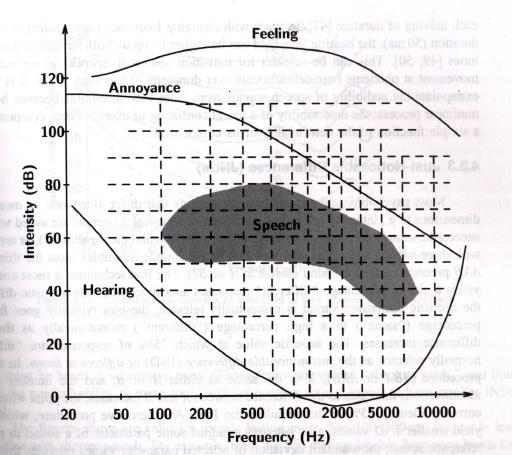
\includegraphics[scale=0.5]{speech_range.jpg}
\end {center}


\newpage
\subsection{Mel scale}

How we perceive sound, that is completely different matter and topic for long philosophical discussion. However we can help ourselves with some subjective experiments. For example Stevens, Volkman and Newman conducted an experiment on a number of listeners to measure, what do we perceive as equally distanced pitches. In this experiment, the participants of the experiment were asked to judge if given pitches were in equal distances. The output was, that humans don't experience sound linearly respectively to the frequency scale, but a perceptual scale was closer to logarithmic one. [5] \newline

Certain formulas were conceived to translate frequency scale to one, that is closer to how human actually perceive sound. \newline

One popular is mel scale, where mel comes from melody: [6] \newline
\begin{equation}
    m = 2595log_{10}(1 + \frac{f}{700})
\end{equation}
	
What looks like that:
\begin{center}
    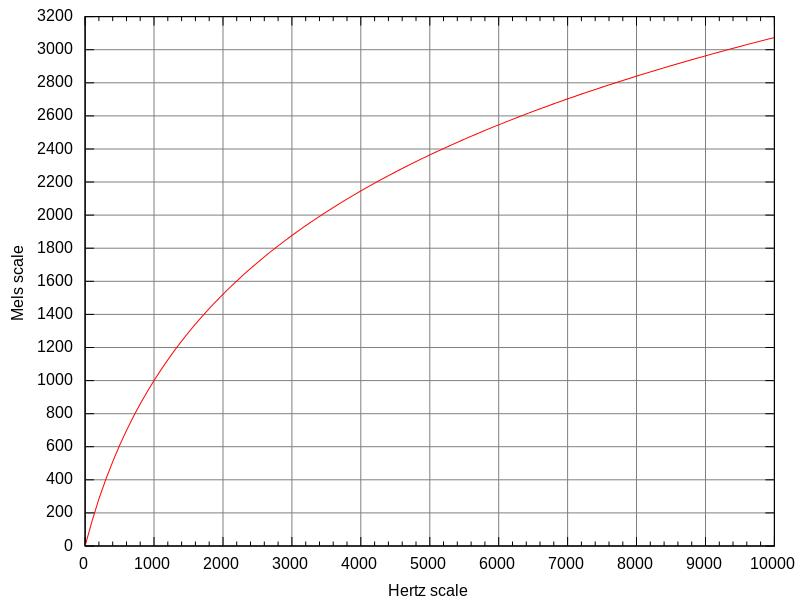
\includegraphics[scale=0.3]{mel_scale.jpg}
\end {center}

Another popular formula of so called bark scale, which is based on perception of loudness of the sound and proposed by Eberhard Zwicker in 1961. [7] \newline
\begin{equation}
    Bark = 13 atan(\frac{0.76f}{1000}) + 3.5 atan(\frac{f^2}{7500^2})
\end{equation}
In this project we use mel scale implemented in sphinx library, although bark scale is becoming more popular recently.

\newpage
\subsection{Frequency spectrum}

The conclusion from the anatomy of human ear is, that frequencies of the sound are important.
How can we obtain frequency spectrum from a digitized sound, so we can proceed further? \newline
The obvious tool for conversion of discrete function to frequencies is Discrete Fourier Transform, named after Jean Baptiste Joseph Fourier it is one of the most often used techniques of modern times. \newline

It all started from the postulate, that a heat equation can be satisfied by function of form: [11] \newline
\begin{equation}
    f(x)=\sum_{n=0}^N(A_n cos(nx) + B_n sin(nx))
\end{equation}
or in complex form:
\begin{equation}
    f(\theta)=\sum_{n=-\infty}^{\infty} C_n e^{i n \theta}
\end{equation}

Basically we convert our function's domain to frequency domain or to domain of sinusoidal functions. $C_n$ coefficients are complex values that encode both amplitude and phase of the converted signal/function at each frequency. \newline

The coefficients for any integrable functions over an interval $[\frac{-T}{2}, \frac{T}{2}]$ can be obtain using formula: [11] \newline
\begin{equation}
    C_n=\int_{\frac{-T}{2}}^{\frac{T}{2}} f(x) e^{-2 \pi i \frac{n}{T} x} dx
\end{equation}

or for the discrete case:
\begin{equation}
    C_k=\sum_{n=0}^{N-1} x_n e^{\frac{-2 \pi i k n}{N}} dx
\end{equation}
	

So far we haven't found any use in the speech recognition for phase part of the coefficients, however amplitude determines how powerful is signal at given frequency. The power value is given by:
\begin{equation}
    |X_k|/N = \sqrt{\Re(X_k)^2 + \Im(X_k)^2} / N
\end{equation}

\newpage
A sample conversion:
\begin{center}
    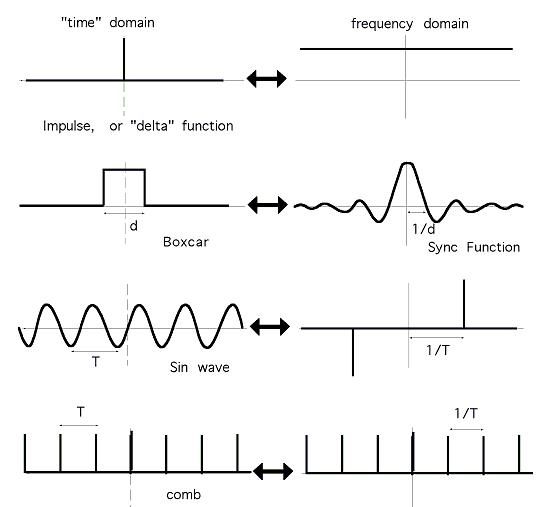
\includegraphics[scale=0.3]{sample_dft_conversion.jpg}
\end {center}

What size of the window should we use? First we have to notice, that in order to capture certain frequency, the window needs to be large enough. We would like to examine signals of frequency ranged from 100Hz (see speech frequencies ranges in chapter 2.1), which is a period of 100th of the second, so a 10millisecond window would be our bottom limit. \newline

Also windows with abrupt signal discontinuities may cause result with spectral artefacts, so a windowing function is usually applied. Popular choice is a Hamming window function: [8]
\begin{equation}
   w_j = 0.54 - 0.46 cos(\frac{2 \pi j}{W - 1}) 
\end{equation}
Which's plot is:
\begin{center}
    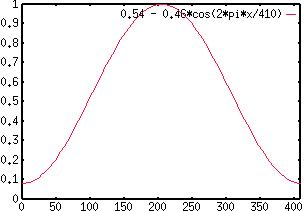
\includegraphics[scale=0.3]{hamming_window.jpg}
\end {center}

Note that it emphasises values in the middle of the window, so our actual windows should overlap to cover whole time domain. For example by shifting a window by a percentage of it actual width:
\begin{center}
    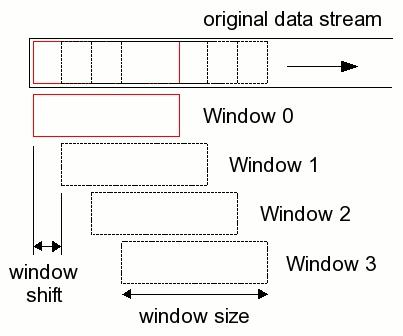
\includegraphics[scale=0.3]{window_shifting.jpg}
\end {center}

\newpage
A human speech signal in frequency and time domain: [3]
\begin{center}
    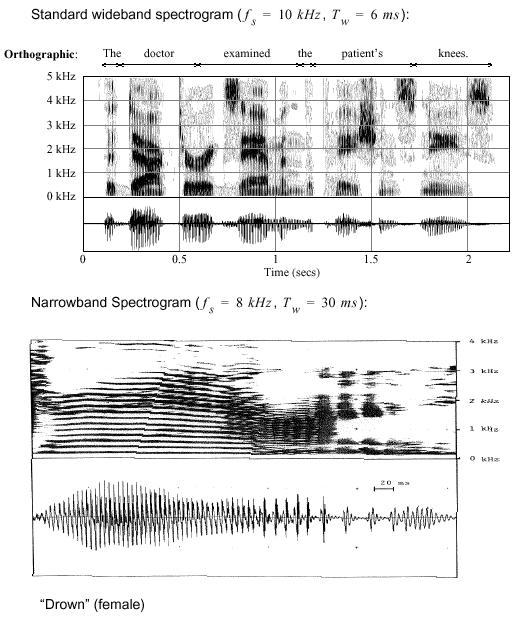
\includegraphics[scale=0.8]{speech_spectrogram.jpg}
\end {center}

\newpage
\subsection{Cepstrum}

Looking at the frequency spectrum of human speech we see, that  the signal in the frequency domain contain features that are quite periodic. As it is with converting initial signal with DFT, we would like to extract the information of periodicity in the spectrum. 
A cepstrum of the signal gives us this additional information. \newline

The word is derived by reordering characters in the word spectrum to indicate switch of domains, similarly as word 'quefrency'. The cepstrum operates in the domain of time and the basic intuition is, that it reveals a rate of change in the different spectrum bands. 
For example a cepstrum of an echoed signal in the picture below shows clearly a three 'quefrencies' of the echo of the signal. [12]
\begin{center}
    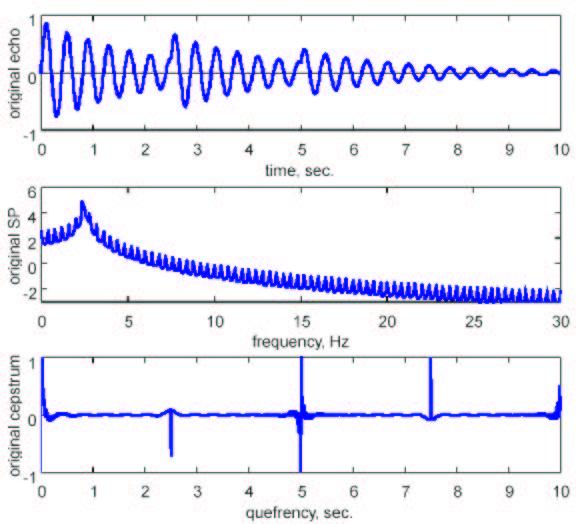
\includegraphics[scale=0.4]{echo_cepstrum.jpg}
\end {center}


Cepstrum definition is: "Inverse Fourier transform of the logarithm of the magnitude of the Fourier transform" or:
\begin{equation}
    C=|F^{-1}{log(|F{f(t)}|^2)}|^2
\end{equation}

,or:
\begin{equation}
    c_x[n] = \frac{1}{2\pi} \int_{-\pi}^{\pi}log |X(e^{j \omega})| e^{j \omega n} d\omega
\end{equation}

This is the definition of the power cepstrum, since it is calculated from the magnitude of each frequency band. However there also exists a complex, real and phase cepstrum depending on what part of initial Fourier transform it uses.
In speech related problems a power cepstrum is usually used and I haven't see any reason to not focus only on this.


\newpage
\addtolength{\textwidth}{4cm}
This is a typical cepstrum sequence of the vowel [3] computed every 10ms. \newline

\begin{minipage}[-100,0]{5cm}
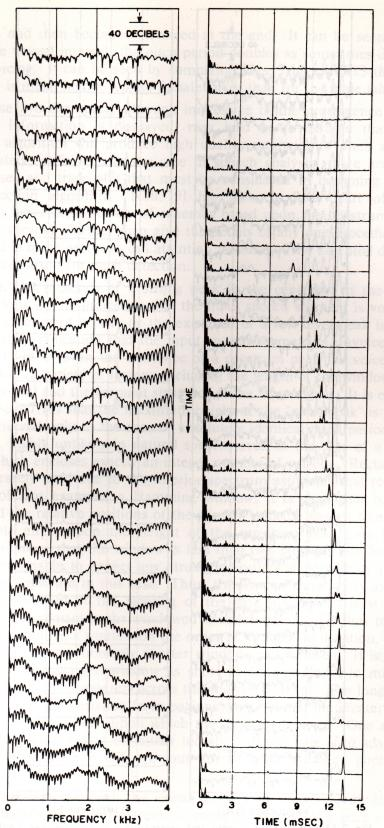
\includegraphics[width=5cm,height=21cm]{vowel_cepstrum.jpg}
\end{minipage}
\begin{minipage}[5cm,0]{9cm}

If the sound becomes periodic in the frequency domain it's quefrency domain contains a peak which is related to the periodicity of the sound. \newline

Note that similar results can be obtained by taking just additional DFT of the signal. Inverse Fourier Transform is closely related to Fourier Transform and also performs a split of the function into periodic components. \newline
\newline
After all IFT is defined:
\begin{equation}
     f(x) = \int_{\mathbb{R} ^ n} e^{2 i \pi x \zeta} \hat{f}(\zeta) d\zeta
\end{equation}
while FT is defined: 
\begin{equation}
    \hat{f}(\zeta) = \int_{\mathbb{R} ^ n} f(x) e^{-2 i \pi \zeta x} dx
\end{equation}

Why taking logarithm of the magnitude? It serves as a normalization of power spectrum. In speech for example it happens, that low frequency components are usually more powerful than high frequncy components and by normalizing the signal, the periodicity becomes more apparent. \newline


A bit different way of looking at the signal cepstrum is as a homomorphic transformation which changes convolution into sum. [3]
\begin{equation}
x(n) = e(n) * h(n)
\end{equation}
\begin{equation}
\hat x(n) = \hat e(n) + \hat h(n)
\end{equation}


Which on it's own can be seen as way of separating signals, since it is more easy to extract elements from a sum, than from a convolution.
\newline
\newline
In the example with echo, we could have used the cepstrum to separate echoed signal from initial signal, and it might be used to filter out an audio feedback.

\end{minipage}

\newpage
\subsection{Sphinx frontend}


Sphinx is a speech recognition toolkit with a lot of useful functionalities for any speech related problem.  \newline
There is a certain common way to prepare a speech signal for the further processing. With slight variations in each step, the useful informations about speech are drawn from a cepstrum of the reduced signal (in the number of data dimensions), as presented in this chapter. \newline

In order to skip the reinvention of the wheel, I used the fronted part of the sphinx library in any experiment in this project.
The sphinx fronted performs signal transformation and produces data composed of only 39 voice features,
while actually only 13 are base ones and the rest is a derivation of these. \newline

Sphinx frontend is a list of transformations executed on the result of the transformation placed higher in the list.
In another words it is a transformation composition. \newline
\newline
This Sphinx frontend pipeline includes: \newline
\begin{itemize}
	\item Data Blocker,
	\item Preemphasizer,
	\item Windower,
	\item Discrete Fourier Transform,
	\item Mel Frequency Filter Bank,
	\item Discrete Cosine Transform,
	\item Cepstral Mean Normalization,
	\item Deltas Feature Extractor.
\end{itemize}

\subsubsection{Data Blocker}

This initial transformation reads incoming double data read from audio source (file or microphone) and
prepares blocks of the data to be used in later phases. In our case blocks contain 10ms of audio data.

\subsubsection{Preemphasizer}

The Preemphasizer applies a formula: $Y[i]=x[i]-(X[i-1] * preemphasizerFactor)$.
The purpose of this transformation is to emphasize the high frequency components. It is kind of filter,
which allows high frequency components to pass through, but weakens the low frequency ones.


\newpage
\subsubsection{Raised cosine windower}

Creates windows from the incoming data. A windowing function
\begin{equation}
    W(n)=(1-\alpha) - \alpha cos(\frac{2 \pi n}{N - 1})
\end{equation}
 is applied afterwards. Alpha coefficient set to 0.46 results with a mentioned before Hamming windowing
 function, which is a default setting and the one used by me.

\subsubsection{Discrete Fourier Transform}

Implementation of fast Fourier transform .The FFT can perform transformation with complexity $\Omega(Nlog(N))$,
where N is the size of the input data.
It can be perform on whole data, however in speech we would like to get an information of the frequencies 
of a small frame, that contains consistent speech signal, in particular a single phoneme.
The output data is the power spectrum of input data window and the complex/phase information is lost.
The number of FFT points is the closest power of 2 equal or larger to the number of samples in the incoming window of data. However the input signal is real, so resulting FFT is symmetric, so only half of the data is returned and the output size is $\frac{FFT points}{2} + 1$.

\subsubsection{Mel frequency filter bank}

This step is a part of calculating a Mel Frequency Cepstrum. \newline

Conversion of frequency spectrum into a mel-spectrum using triangular overlapping windows defined as:
\begin{equation}
    w(n) = 1 - |\frac{n - (N - 1)/2}{(N + 1)/2}|
\end{equation}


The number of triangles/filters defined the size of mel-spectrum and the sphinx's default is 40. \newline
The filters are chosen, so the result would simulate a mel-scale given by the formula:
\begin{equation}
    melFreq = 2595 log(1 + linearFrequency / 700)
\end{equation}

The given filters should look like in the picture:
\begin{center}
    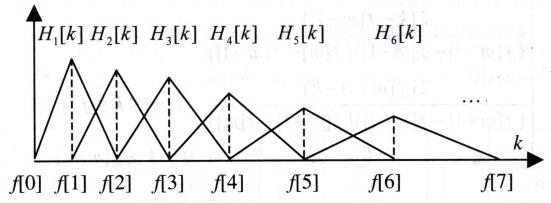
\includegraphics[scale=0.4]{mel_filters.jpg}
\end {center}

Not all frequencies are covered by the filters.
The chosen range of frequencies may differ for various audio encodings,
but generally should cover only the speech ranges.
The default values for 16kHz sample rate streams are 130Hz-6800Hz and are not changed in this project.

\newpage
\subsubsection{Discrete Cosine Transform}

Another part of calculating Mel Frequency Cepstral Coefficient vector.  \newline

It applies a logarithm and the DCT type II to the input data.  \newline

A DCT type II (most common) coefficients are defined as: 
\begin{equation}
    C(u) = \alpha(u)\sum_{x=0}^{N-1} f(x)cos[\frac{\pi(2x+1)u}{2N}] 
\end{equation}
and it is quite tightly related to real part of the Fourier Transform. [18]
The transform represents a function as a sum of cosine functions and it is equivalent to the DFT operating
real data with even symmetry. \newline
The number of dimensions returned is set by default to 13.

\subsubsection{Cepstral Mean Normalization}

Performs a normalization of MFCC vector by subtracting a mean of all the input. There are two versions
of this step. One that calculates mean online and the other that reads all data before performing
subtraction.

\subsubsection{Deltas feature extractor}

The final transformation in the sphinx frontend chain. It calculates first and second order derivative of the
cepstrum as additional features of the speech signal. It improves noticeable speech processing algorithms
by adding additional information about changes in the cepstrum data. \newline

For the initial cepstrum data it adds additionally twice the size vector with first and second order
differences, calculated as shown in the picture:
\begin{center}
    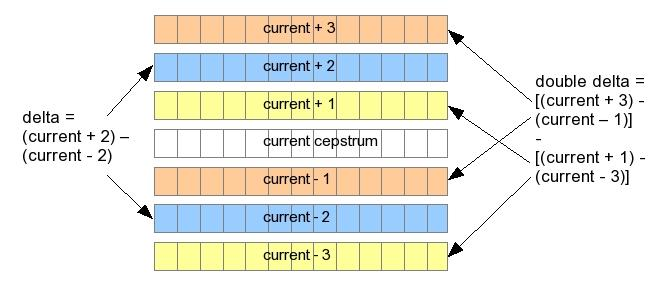
\includegraphics[scale=0.6]{deltas_calc.jpg}
\end {center}

\newpage
\begin{center}
    \section{Speech Modelling}
\end {center}
\setcounter{equation}{0}

\subsection{Phones, phonemes and graphemes}

A phone is a unit of speech sound [20]. Phoneme's definition is: "The smallest contrastive linguistic unit, which may bring about a change of meaning" [21], so the phoneme is a classification unit of phones, which allow us to represent speech while preserving its meaning.  While speech is being modelled using phonemes the graphical part of the language in form of text is modelled with characters or graphemes. \newline

Language grapheme set usually differs quite substantially from it audio counterparts. Often it contains more characters than needed to represent every word from given language and at the same time it is much too small to represent all the nuances of human speech. What is more problematic, the word graphic representation often has very little to do with actual phones of the word. I.e. there are so called homographes: words, that are written the same yet they pronunciation differs ("zamarzać" from "marznąć" and "morzyć") or homophones, that look differently, but are pronounced similar ("może", "morze"). In polish though, the former is quite rare and this fact is actually used by me (chapter 5.3). \newline


Actual phones that are classified under single phoneme create a diversified family.  Different variants of a phoneme are called allophones. For example /l/ in English "leap" and "deal" or polish examples of allophones (/ł/ in "umysł" might be soundless contrary to "ławka") or vowels between soft consonants (/a/ in "jajko"). [22] \newline

The phonemes can differ quite substantially depending on the surrounding phones. For example almost each phoneme in polish changes to softer version when put next to /i/ or /j/. Consecutive phones are not necessarily separated by clearly visible moment of silence. Often one phone is converting slowly into another. To model such a transitions a diphones or triphones are modelled for each sequence of two or three phones. \newline

Phonemes are very important in the computational language modelling, either in speech recognition or alignment. The importance is derived directly from its definition. It is a unit of speech, which can't be switched to another without changing the meaning. This is the unit, that need to be modelled if we want to recognize and/or distinguish different words. Finer granularity of model is necessary only to make a better prediction where an observed phone belongs.

\newpage
Some of English phonemes and example phones:
\begin{center}
    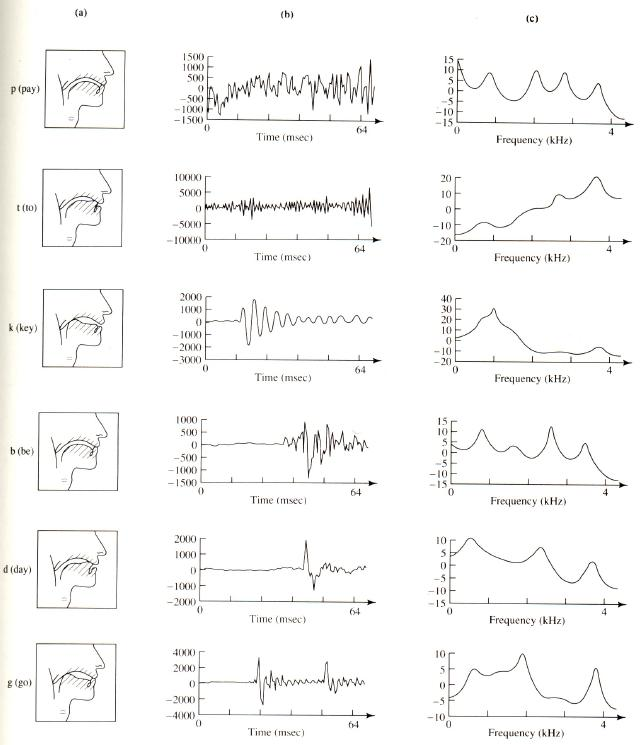
\includegraphics[height=11cm, width=16cm]{example_phones_1.jpg}
    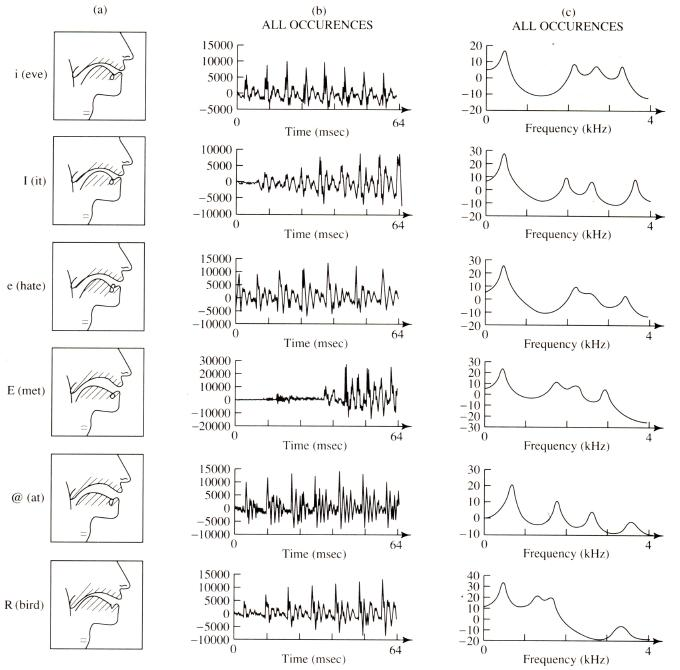
\includegraphics[height=11cm, width=16cm]{example_phones_2.jpg}
\end {center}

\newpage
\subsection{Audio distances}

The simplest way to find similar audio sequence is to find a sequence which is nearby to another,
that we know represents a certain sound, phoneme or word. \newline

To calculate a distance we could use various norms:
\begin{equation}
    ||x||_1 , || x ||_2, ... , || x ||_\infty
\end{equation}
, where 
\begin{equation}
    ||x||_k = (\sum_{i=0}^{N} x_i^k)^\frac{1}{k}
\end{equation}
and they are all fine for uncorrelated vectors, which is not really our case. \newline


For correlated vectors, we could try to introduce some weighting factor inside.\newline
What factor should we use?\newline
One approach is to tune the factors using external methods, which theoretically may give us some additional benefit of properly modelling phonemes, that we try to measure distance from, however this is a bit out of the scope of this chapter and most probably would in the end look similar to a different method.
A simpler approach would be to calculate correlations and use them in a distance measure.
If we had a correlation matrix ($P$) and than our distance could be:
\begin{equation}
    dist_{using correlations}(\vec x, \vec p) = (\vec x - \vec p)^T P^{-1} (\vec x - \vec p)
\end{equation}
               
Karl Pearson introduced such an idea [23] in form of correlation coefficient defined between two random populations:  
\begin{equation}
    \rho_XY = \frac{cov(X, Y)}{\sigma_X \sigma_Y} = \frac{E[(X - \mu_X)(Y - \mu_Y)]}{\sigma_X \sigma_Y}
\end{equation}
and in the form of matrices:  
\begin{equation}
    P = (\Sigma^{diagonal})^{-1/2} \Sigma (\Sigma^{diagonal})^{-1/2}
\end{equation}

It should be noted, that in the denominator we have standard deviations which don't really bring any value to our measure, since this is a constant factor.
By removing them we obtain so called Mahalanobis distance [16]:
\begin{equation}
    distance_{Mahalanobis}(\vec x, \vec p) = (\vec x - \vec p)^T \tilde C^{-1} (\vec x - \vec p)
\end{equation}

If we knew elements belonging to any given phoneme, we could calculate a distance between this training sample and any encounter speech signal.

\newpage

I conducted couple of experiments with different distances.
Starting with a flawed alignment of larger portions of text I tried to:
\begin{itemize}
	\item find the same word, that is quite lengthy and occurs multiple times just by searching for similar sequences,
	\item find a given sequence of three phonemes in a text, based on estimated location (time)
\end{itemize}

Mahalanobis distance in those experiments where not expected to any give significant results,
since there were conducted without knowledge of phone classification and it behaved without a surprise. \newline


The euclidean norm were performing the best. \newline
In the second experiment it was able to find around 50\% of all occurences of three phoneme sequence from beginning of the text and other found were quite similar (80\% of the time they contained two out of three phonemes), although I was lucky, that in my testing recording, the starting three phonemes occurrences later in the text were quite far from each other. \newline


Searching for whole word didn't give me any satisfying results. I could find a similar word when I pointed, which it should have being searched for,
but without the intervention it always found a sequences which weren't similar at all (from a speech point of view) and at the same time the matching words, I was expected to find, were far in the list.

\newpage
\subsection{Gaussian Model}

Given observation points belonging to a single class (a phoneme) with a given probability,
we would like to model a distribution of emitting data point by the class. \newline


A natural choice is a normal distribution, although we have to remember, that observation comes from a multidimensional universum, where populations are not independent. \newline
Luckily there is a definition of multivariate normal distribution, that considers correlations:
\begin{equation}
    f_x(x_1,...,x_k) = \frac{1}{\sqrt{(2\pi)^k |{\Sigma}| }}exp(-\frac{1}{2}(x-\mu)^T{\Sigma}^{-1}(x-\mu))
\end{equation}
                       
where $\Sigma$ is a covariance matrix and $|\Sigma|$ is its determinant. \newline


Covariance matrix is always symmetric and positive-semidefinitive.\newline
Symmetry comes directly from a definition: $cov(X) = E[(X - E(X))(X - E(X))^T]$, since outer product of a single vector gives always a symmetric matrix. \newline

Positive-semidefinitive matrix is a matrix, where for any product $a^T A a$ with any non-zero complex vector $a$ is real and non-negative:
\begin{equation}
    a^T A a >= 0
\end{equation}

A product with any vector $a$ and covariance matrix is also equal to: 
\begin{equation}
    a^T \Sigma a = a^T E(XX^T) a + a^T\mu\mu^T a = \frac 1 N (\sum_{i=1}^N a^T X X^T a) + a^T\mu\mu^T a
\end{equation}
and each element of the sum is square of inner product of two vectors, so it is always positive (or equal to zero). \newline

In order to prevent degenerate cases we can allow only positive-definite matrices. \newline
Any such a matrix is guaranteed to be invertible. \newline


If the number of dimensions is equal to one, then the formula reduces to single-variable normal distribution: 
\begin{equation}
    f(x) = \frac 1 {\sqrt{(2\pi)}\sigma}e^{-{ \frac {(x-\mu)^2}{2 \sigma^2}}}
\end{equation}


\newpage

A normal distribution of emitting signal frame have two free parameters: a mean vector and a covariance matrix,
which needs to be calculated.\newline
I assume, that an input is the list of observations with assigned probability.\newline 

If probability is actually a likelihood of emitting the signal (or its estimation),
than we can calculate mean with a formula:   
\begin{equation}
    \vec \mu = \sum_{\vec X} Pr(\vec X) \vec X
\end{equation}
and a covariance matrix by: 
\begin{equation}
    \hat C = \sum_{vec X} Pr(\vec X) (\vec X - \mu) (\vec X - \mu)^T
\end{equation}
\newline


In the case, that probability is not a direct likelihood of given point, but a conditional probability of emitting the signal,
(i.e. under the condition that it belongs to given sequence), the probabilities need to be normalized first. \newline

We can assume, that conditional probability is the same for each observation,
 so the input probability is in the form of $ Pr(\vec X) Pr_{condition}$,
then they have to be divided by a total sum to produce actual likelihood:
\begin{equation}
    Pr(\vec X) = \frac{Pr_{input}(\vec X)}{\sum_{\vec X} Pr_{input}(\vec X)} = \frac{Pr(\vec X) Pr_{condition}}{\sum_{\vec X} Pr(\vec X) Pr_{condition}} = 
\frac{Pr(\vec X)}{\sum_{\vec X} Pr(\vec X)}
\end{equation}

The denominator should sum to 1, after all it is a probability of emitting given point under a condition, that only $|X|$ points were emitted.

\newpage
\subsection{Expected-Maximization algorithm}

Expected-Maximization method is a technique for estimating parameters of any underlying distribution based on observed data. It tries to maximize the likelihood, that the data would be observed by the distribution: 
\begin{equation}
    argmax_{\theta} Pr(X | \theta)
\end{equation}

For certain distribution parameters, that maximize likelihood of the data, can be solved, i.e. calculated mean vector and variance are parameters to normal distribution, that do maximize the likelihood of observing the observation data.
We can calculate a derivative of normal density function to show it:


what is a definition of a mean,


what is a definition of variance and standard deviation is a square root of variance.
And similarly can be done for many other distributions, including multivariate normal distribution.

It is not always the case, that one can calculate parameters so easily, i.e. mixture models of several populations may not give so easily.
Let's consider a mixture of Gaussian models of some populations. We have a random population, where each point is randomly drawn from each distribution. 
So the total likelihood of any point is: , where is a probability of drawing a point from ith distribution and  is a density function of ith model.

Since each model from a mixture is easily solvable, if we knew to which model each point belonged, than estimating parameters would be easy, or at least what is the probability, that given point was drawn from a given class (see chapter about Gaussian model).


\end{document}
